\chapter{Data Exploration}
\label{chap:data exploration}

\section{Database Composition}
\label{sec:database composition}

The database was originally composed on a popular spreadsheet program and stored in a comma separated value file (.csv).  There are pros and cons to using spreadsheets.   Spreadsheets are very simple and easily understood tools for data entry, retrieval, and analysis.   The programs are easily obtainable and the data structure is easily modifiable as the new data types are added.  Yet, from my experience, they can be more prone to typographical errors and misplacing of data than other more formal database systems.  Yet, in-spite of the possible errors it was determined that simplicity of use was the most important factor.

Data was arranged in the database such that each row corresponded to one sample set and each column corresponded to a data type.  An example of a spreadsheet is shown in figure \ref{fig:spreadsheetExample}.  This figure is a screen-shot of a spreadsheet.  It does not show the breadth or depth of the data set, but is intended to show enough detail to assist in understanding the spreadsheet format.  Promotion of any particular spreadsheet program is not intended or implied in this figure.

\begin{figure}
	\centering
	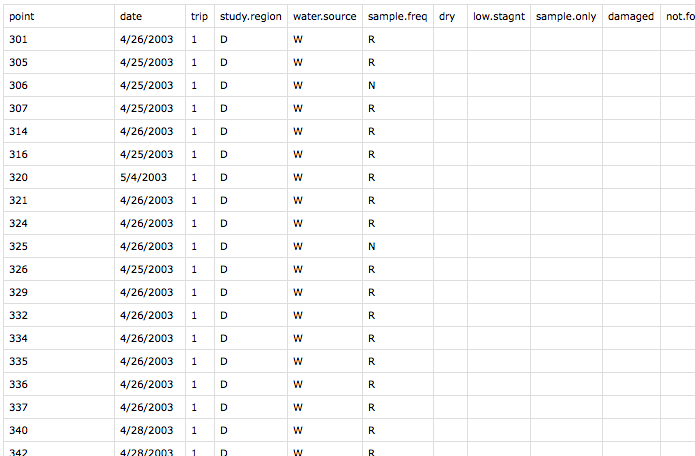
\includegraphics[width=6in]{Figures/Photo/ExampleDatabaseSpreadsheet}
	\caption[Example database spreadsheet.]{Example database spreadsheet.}
	\label{fig:spreadsheetExample}
\end{figure}	

Data analysis should begin with a simple exploration of the database.  This exploration consists of a review of the data points and data types.  The results allow for the re-organization of the database into a form that is acceptable to the software used for statistical analysis and that includes only the relevant data points and data types.  

 A significant number of the columns in the original spreadsheets were intended for centralized book-keeping of results and not for data analysis.  Therefore, a trimmed copy of this spreadsheets were made where columns not intended for data analysis were removed.  The original spreadsheets also included data points (rows) that were not relevant to this investigation.  These rows were removed.

One of the cleaned spreadsheets contained the data columns and types as shown in table \ref{tab:trimmedData}.  This spreadsheet's primary contents are the selenium concentration lab results.  The other spreadsheet was used to contain all of the continuous data obtained from the USGS and CDWR.  This data set contained the data columns and types show in table \ref{tab:continuousData}.  The continuous data spreadsheet was divided into two separate files based on the study region.

\begin{table}[htbp]
	\centering
	\caption[Trimmed Data Set.]{Trimmed Data Set.}
	\label{tab:trimmedData}
	\begin{tabular}{l  l  l}
		\toprule
		Column & \multirow{2}{*}{Type}  & \multirow{2}{*}{Description}\\
		Name
		\\ \toprule
		point & string & Name of the data point location.\\
		date & string & Date the sample was taken using the format mm/dd/yyyy. \\
		se & numeric & Selenium concentration. \\
		se.d & numeric & Selenium concentration duplicate sample.
		\\ \bottomrule
	\end{tabular}
\end{table}

\begin{table}[htbp]
	\centering
	\caption[Continuous Data Set.]{Continuous Data Set.  Column names with italic letters denote multiple columns where each column corresponds to a different location. }
	\label{tab:continuousData}
	\begin{tabular}{l  l  l}
		\toprule
		Column & \multirow{2}{*}{Type}  & \multirow{2}{*}{Description}\\
		Name
		\\ \toprule
		date & string & Date the sample was taken using the format mm/dd/yyyy. \\
		q.in & numeric & Water flow rate at the region inlet gauge. \\
		ec.in & numeric & Specific conductivity at the region inlet gauge. \\
		t.in & numeric & Water temperature at the region inlet gauge. \\
		q.\textit{x} & numeric & Water flow rate at gauge \textit{x}. \\
		q.out & numeric & Water flow rate at the region outlet gauge. \\
		ec.out & numeric & Specific conductivity at the region outlet gauge. \\
		t.out & numeric & Water temperature at the region outlet gauge. \\
		d.\textit{y} & numeric & Calculated average flow depth for segment \textit{y}. \\
		p & numeric & The day's reported precipitation. \\
		et & numeric & The day's reported average evapo-transpiration. \\
		rhmin & numeric & The day's reported minimum relative humidity. \\
		u2 & numeric & The day's reported wind velocity at \SI{2}{\meter} above ground surface. 
		\\ \bottomrule
	\end{tabular}
\end{table}

Data exploration is simplified when all of the relavent data points are contained within one document.  In our case, we have two files that are organized on different schemes; one with each row corresponding to a collected sample and the other with each row corresponding to a day.  We needed to combine the two spreadsheets into one file to simplify any further analysis.  Both spreadsheets contained the variable (column name) "date".  The new, combined spreadsheet was organized from the simplified spreadsheets such that it contained the columns as described in table \ref{tab:combinedData}.  As before, there are two separate spreadsheets with the data corresponding to the study region.  Within each of the combined tables, there were multiple rows where there were data was not available for a particular variable (column).  It was determined that all variables were necessary to provide a sufficient analysis of the complete data set.  In these cases, the row was removed.  Exceptions were made in cases where selenium samples were collected on sequential days.  All surface water samples for either of the study regions could be obtained within a 24 hour period.  This lag in sample collection time is considered well within acceptable range considering the size of the study regions.  In these cases, the date for the sample with the varying date was changed to match that of the majority of samples collected during that sampling event/trip.

\begin{table}[htbp]
	\centering
	\caption[Combined Data Set.]{Combined Data Set.  Column names with italic letters denote multiple columns where each column corresponds to a different location. }
	\label{tab:combinedData}
	\begin{tabular}{l  l  l}
		\toprule
		Column & \multirow{2}{*}{Type}  & \multirow{2}{*}{Description}\\
		Name
		\\ \toprule
		date & string & Date the sample was taken using the format mm/dd/yyyy. \\
		q.in & numeric & Water flow rate at the region inlet gauge. \\
		ec.in & numeric & Specific conductivity at the region inlet gauge. \\
		t.in & numeric & Water temperature at the region inlet gauge. \\
		q.\textit{x} & numeric & Water flow rate at gauge \textit{x}. \\
		q.out & numeric & Water flow rate at the region outlet gauge. \\
		ec.out & numeric & Specific conductivity at the region outlet gauge. \\
		t.out & numeric & Water temperature at the region outlet gauge. \\
		d.\textit{y} & numeric & Calculated average flow depth for segment \textit{y}. \\
		p & numeric & The day's reported precipitation. \\
		et & numeric & The day's reported average evapo-transpiration. \\
		rhmin & numeric & The day's reported minimum relative humidity. \\
		u2 & numeric & The day's reported wind velocity at \SI{2}{\meter} above ground surface. \\
		se.\textit{z} & numeric & Selenium concentration at point \textit{z}.
		\\ \bottomrule
	\end{tabular}
\end{table}

After merging the spreadsheets and cleaning up the data, a statistical summary of the data was produced with R for both regions.  These summaries, shown in figures \ref{fig:mineSummaryUS} and \ref{fig:mineSummaryDS} for the upstream study reach and the downstream study reach, respectively, present the minimum, first quartile, median, mean, third quartile, maximum, and quantity of any missing values for each variable.

\begin{figure}
	{
		\setstretch{1.0}
		\tiny{
			\VerbatimInput{Tables/mineSummaryUS.txt}
		}
	}
	\caption[Combined Data Summary - Upstream Study Region.]{Combined Data Summary - Upstream Study Region.}
	\label{fig:mineSummaryUS}
\end{figure}

\lipsum[1]

\begin{figure}
	{
		\setstretch{1.0}
		\tiny{
			\VerbatimInput{Tables/mineSummaryDS.txt}
		}
	}
	\caption[Combined Data Summary - Downstream Study Region.]{Combined Data Summary - Downstream Study Region.}
	\label{fig:mineSummaryUS}
\end{figure}

\lipsum[1]

\clearpage{}